\chapter{Pulse Wave Solver}

\section{Synopsis}

The PulseWaveSolver solves the nonlinear hyperbolic system
(Equ.~\ref{e:pulsewave:hyperbolic}) based on the variables $(A,u)$ and is
directly obtained by conservation of mass and momentum for a $1$-dimensional
domain.

\begin{subequations}
\begin{align}
\frac{\partial A}{\partial t} + \frac{\partial A u}{\partial x} &= 0 )]] \\
\frac{\partial u}{\partial t} + u \frac{\partial u}{\partial x} + \frac{1}{\rho}
\frac{\partial p}{\partial x} + K_R u&= 0 
\label{e:pulsewave:hyperbolic}
\end{align}
\end{subequations}

The reduction of three-dimensional flow towards one dimension is achieved by
assuming the flow is constant over the cross- sectional area. This assumption
allows an accurate representation of the in-vivo environment at a reasonable
computational cost \cite{ShFoPeFr03}. In the following, we will explain
the usage of the blood flow solver on the basis of a single-artery problem and
also on an arterial network consisting of $55$ arteries.

\section{Usage}
\begin{lstlisting}[style=BashInputStyle]
PulseWaveSolver session.xml
\end{lstlisting}

\section{Session file configuration}

\subsection{Session Info}
The PulseWaveSolver is sqpecified through the \inltt{EquationType}
option in the session file. This can be set as follows:
\begin{itemize}
\item \inltt{Projection}: Only a discontinuous projection can be specified
using the following option:
    \begin{itemize}
    \item \inltt{Discontinuous} for a discontinous Galerkin (DG) projection.
    \end{itemize}
\item \inltt{TimeIntegrationMethod}
\item \inltt{UpwindTypePulse}:
    \begin{itemize}
    \item \inltt{UpwindPulse}
    \end{itemize}
\end{itemize}

\subsection{Parameters}

The following parameters can be specified in the \inltt{PARAMETERS} section of
the session file:
\begin{itemize}
\item \inltt{rho}: sets the density (Default value: 1.0).
\item \inltt{nue}: sets the poisson's ratio (Default value: 0.5).
\item \inltt{pext}: sets the external pressure (Default value: 0.0).
\item \inltt{h0}: sets a constant arterial wall thickness (Default value: 1.0).
\item \inltt{a1}: (Default value: 0).
\item \inltt{a2}: (Default value: 0).
\item \inltt{kappa}: (Default value: 0).
\item \inltt{Y0}: (Default value: 0).
\item \inltt{k}: (Default value: 0).
\item \inltt{k1}: (Default value: 0).
\end{itemize}

\subsection{Functions}
The following functions can be specified inside the \inltt{CONDITIONS} section
of the session file:
\begin{itemize}
\item \inltt{AdvectionVelocity}: specifies the advection velocity $v$.
\item \inltt{InitialConditions}: specifies the initial condition for unsteady
 problems.
\item \inltt{Forcing}: specifies the forcing function $f$
\end{itemize}

\section{Examples}

\subsection{Human Vascular Network}
The Pulse Wave Solver is also capable of handling more complex networks, such as
a complete human arterial tree proposed by Westerhof et al. \cite{We69}.
In this example, we will use the refined data from \cite{ShFoPeFr03} and set up
the network shown in the figure in the right. We will explain how bifurcations
are set correctly and how each arterial segment gets its correct physiological
data.

\begin{figure}
	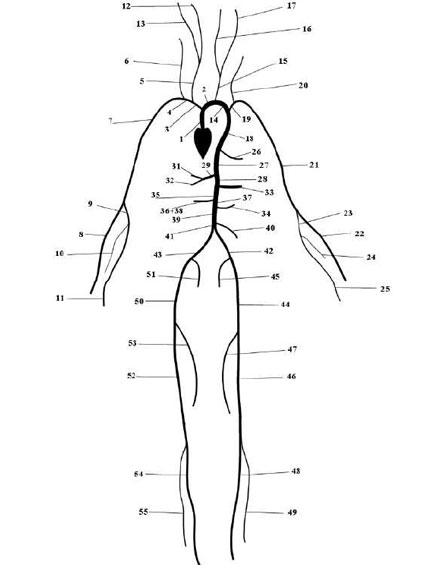
\includegraphics[width=0.49\linewidth]{Figures/55_artery_network.jpg}
	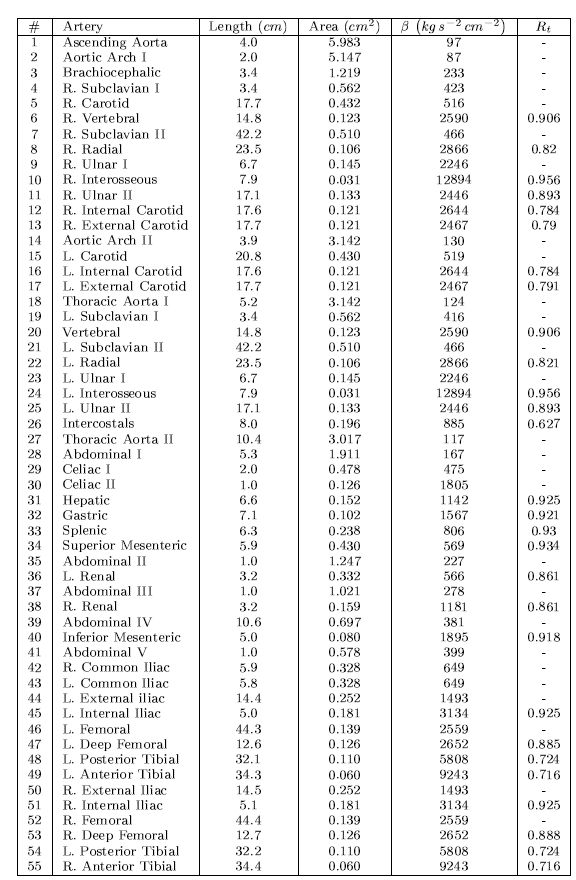
\includegraphics[width=0.49\linewidth]{Figures/Data_Table.png}
\end{figure}

First, we will set up the mesh where each arterial segment is represented by one
element and two vertices respectively. Then, we will subdivide the mesh into
different subdomains by using the \inltt{<COMPOSITE>} section. Here, each
arterial segment is described by the contained elements and its first and last
vertex.

The mesh connectivity is specified during the creation of elements by indicating
the starting vertex and ending vertex of each individual artery segment. Shared
vertices are used to describe bifurcations, junctions and mergers between
different artery segments in the network.

The composites are then used to specify the two adjoining segments of an artery,
where the first segment merely allows for description of the connectivity.

\begin{lstlisting}[style=XmlStyle]
<GEOMETRY DIM="1" SPACE="1">
    <VERTEX>
        <V ID="0"> 0.000e+00 0.000e+00 0.000e+00</V> <!-- 1 -->
        <V ID="1"> 4.000e+00 0.000e+00 0.000e+00</V>

        <V ID="2"> 4.000e+00 0.000e+00 0.000e+00</V> <!-- 2 -->
        <V ID="3"> 6.000e+00 0.000e+00 0.000e+00</V>

        <V ID="4"> 4.000e+00 0.000e+00 0.000e+00</V> <!-- 3 -->
        <V ID="5"> 7.400e+00 0.000e+00 0.000e+00</V>
           .
           .
           .
        <V ID="108"> 109.100e+00 -45.000e+00 0.000e+00</V> <!-- 55 -->
        <V ID="109"> 143.500e+00 -45.000e+00 0.000e+00</V>
    </VERTEX>
    <ELEMENT>
        <S ID="0">    0     1 </S>
        <S ID="1">    1     2 </S>
        <S ID="2">    1     4 </S>
        <S ID="3">    2     3 </S>
        <S ID="4">    4     5 </S>
        <S ID="5">    5     6 </S>
        <S ID="6">    5     8 </S>
        <S ID="7">    6     7 </S>
        <S ID="8">    8     9 </S>
          .
          .
          .
        <S ID="106">   103    108 </S>
        <S ID="107">   108    109 </S>
        <S ID="108">   85    98 </S>
    <ELEMENT>
    <COMPOSITE>
        <C ID="0"> S[0] </C> <!-- 1 -->
        <C ID="1"> V[0] </C>
        <C ID="2"> V[1] </C>

        <C ID="3"> S[1,3] </C> <!-- 2 -->
        <C ID="4"> V[2] </C>
        <C ID="5"> V[3] </C> 

        <C ID="6"> S[2,4] </C> <!-- 3 -->
        <C ID="7"> V[4] </C>
        <C ID="8"> V[5] </C>
           .
           .
           .
        <C ID="162"> S[106,107] </C> <!-- 55 -->
        <C ID="163"> V[108] </C>
        <C ID="164"> V[109] </C>            
    </COMPOSITE>
</GEOMETRY>
\end{lstlisting}

Then the choice of polynomial order, solver information, area of the arteries
and other parameters are specified.

\begin{lstlisting}[style=XmlStyle]
<EXPANSIONS>
    <E COMPOSITE="C[0]" NUMMODES="5" FIELDS="A,u" TYPE="MODIFIED" />
    <E COMPOSITE="C[3]" NUMMODES="5" FIELDS="A,u" TYPE="MODIFIED" />
       ...

    <E COMPOSITE="C[162]" NUMMODES="5" FIELDS="A,u" TYPE="MODIFIED" />
</EXPANSIONS>

<CONDITIONS>

    <PARAMETERS>

        <P> TimeStep       = 1e-4               </P> 
        <P> FinTime        = 1.0              </P>
        <P> NumSteps       = FinTime/TimeStep   </P>
        <P> IO_CheckSteps  = NumSteps/50        </P>
           ...
        <P> A53            = 0.126              </P>
        <P> A54            = 0.110              </P>
        <P> A55            = 0.060              </P>
    </PARAMETERS>

    <SOLVERINFO>
        <I PROPERTY="EQTYPE" VALUE="PulseWavePropagation" />
        <I PROPERTY="Projection" VALUE="DisContinuous" />
        <I PROPERTY="TimeIntegrationMethod" VALUE="RungeKutta2_ImprovedEuler" />
        <I PROPERTY="UpwindTypePulse"  VALUE="UpwindPulse"/> 
    </SOLVERINFO>

    <VARIABLES>
        <V ID="0"> A </V>
        <V ID="1"> u </V>
    </VARIABLES>

\end{lstlisting}

The vertices where the network terminates are specified as boundary regions
based on their subsequent composite ids.

\begin{figure}
	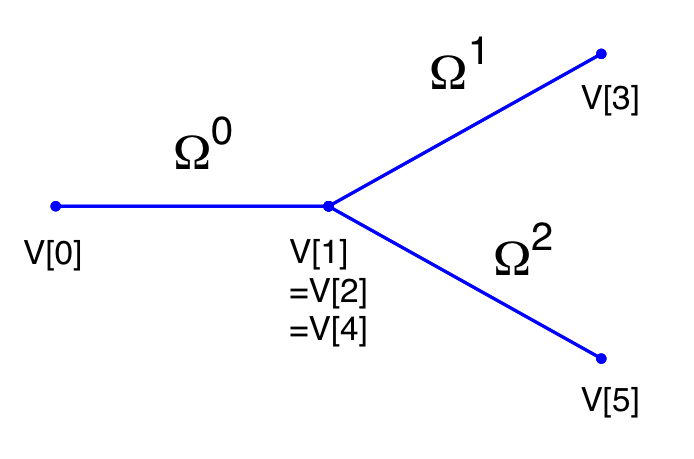
\includegraphics[width=0.49\linewidth]{Figures/Bifurcation.png}
	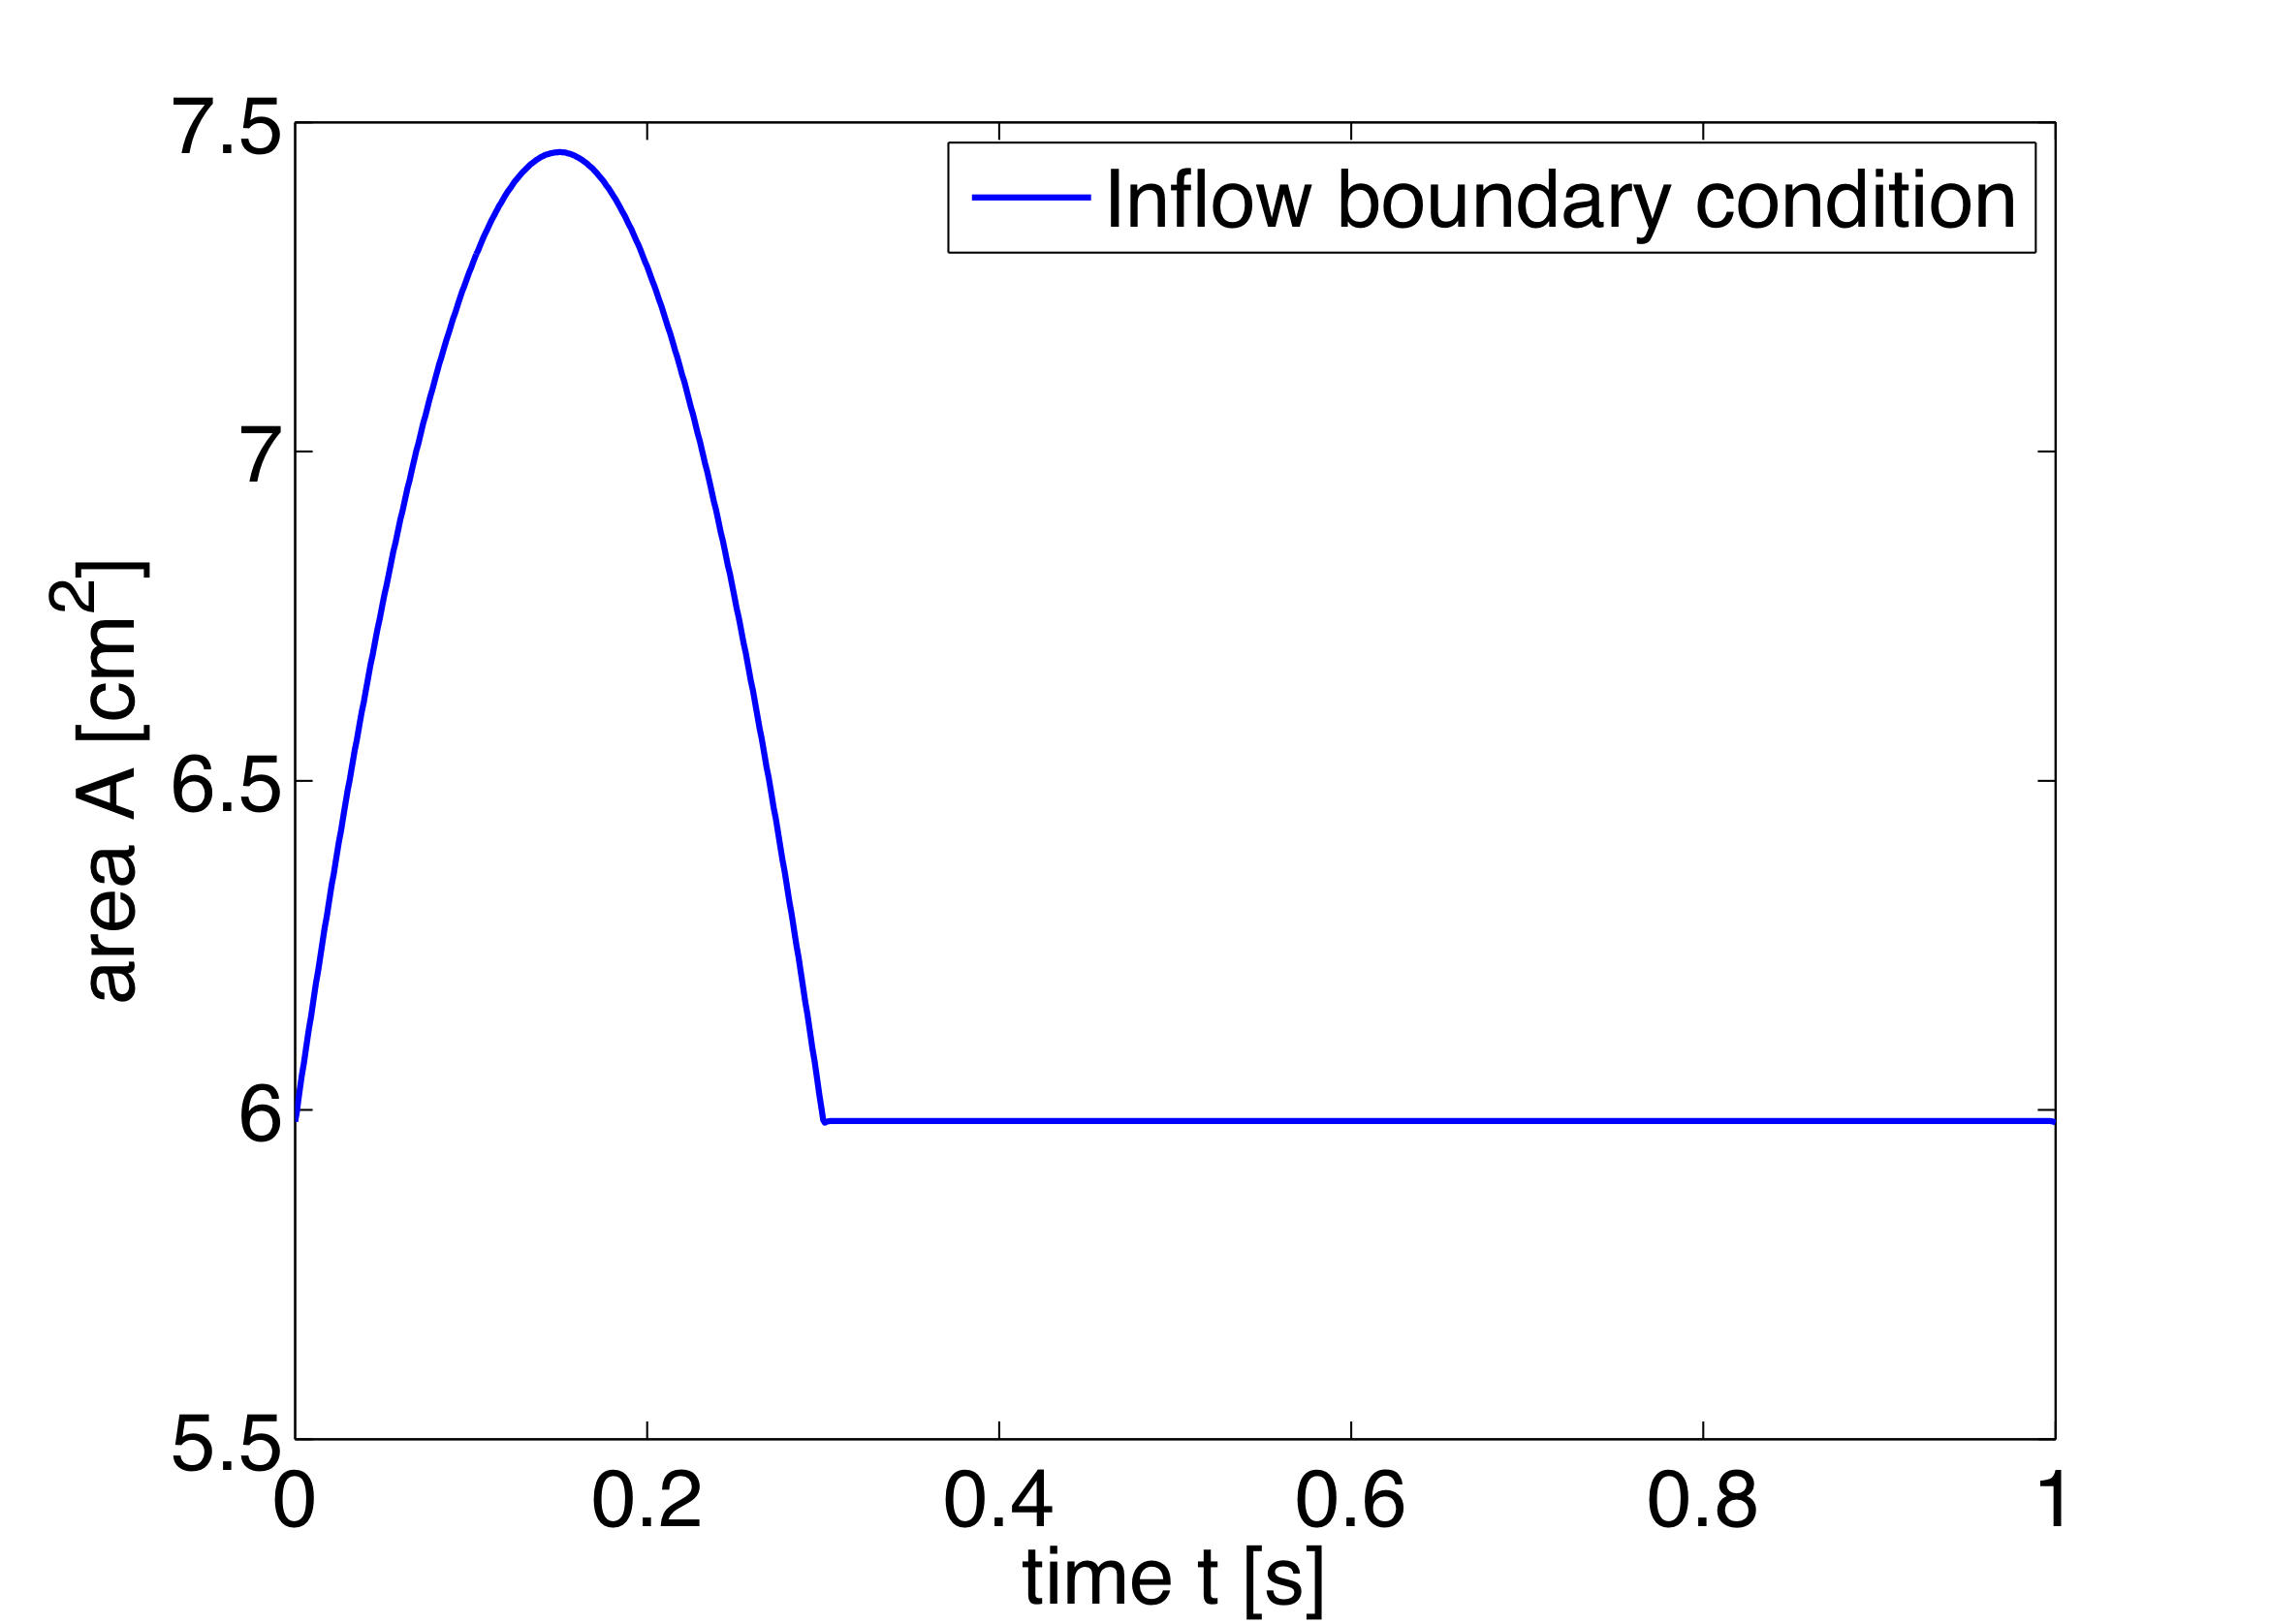
\includegraphics[width=0.49\linewidth]{Figures/Network_Inflow.png}
\end{figure}

\begin{lstlisting}[style=XmlStyle]
        <BOUNDARYREGIONS>
            <B ID="0"> C[1] </B> <B ID="1"> C[17] </B> <B ID="2"> C[23] </B>
               ...
            <B ID="28"> C[164] </B>
       </BOUNDARYREGIONS>
\end{lstlisting}

In the boundary conditions section the inflow and outflow conditions are set up.
Here we use an inflow boundary condition for the area at the beginning of
the ascending aorta taken from \cite{ShFoPeFr03} and plotted on the
right. Potential choices for inflow boundary conditions include Q-Inflow
and Time-Dependent inflow. The outflow conditions for the terminal regions of
the network could be specified by different models including eTerminal, R, CR,
RCR and Time-Dependant outflow.

\begin{lstlisting}[style=XmlStyle]
<BOUNDARYCONDITIONS>
    <REGION REF="0"> <!-- Inflow -->
        <D VAR="A" USERDEFINEDTYPE="TimeDependent" 
           VALUE="5.983*(1+0.597*(sin(6.28*t + 0.628) - 0.588)*
                (1./(1+exp(-2*200*(sin(6.28*t + 0.628) - 0.588)))))" />
        <D VAR="u" USERDEFINEDTYPE="TimeDependent" VALUE="0.0" />
    </REGION>
    <REGION REF="1">  
        <D VAR="A" USERDEFINEDTYPE="TimeDependent"  VALUE="A6" />
        <D VAR="u" USERDEFINEDTYPE="TimeDependent"  VALUE="0.0" />
    </REGION>            
    <REGION REF="2"> 
        <D VAR="A" USERDEFINEDTYPE="TimeDependent"  VALUE="A8" />
        <D VAR="u" USERDEFINEDTYPE="TimeDependent"  VALUE="0.0" />
    </REGION>
    <REGION REF="3">   
        <D VAR="A" USERDEFINEDTYPE="TimeDependent"  VALUE="A10" />
        <D VAR="u" USERDEFINEDTYPE="TimeDependent"  VALUE="0.0" />
    </REGION>
    ....
    <REGION REF="28"> 
        <D VAR="A" USERDEFINEDTYPE="TimeDependent"  VALUE="A55" />
        <D VAR="u" USERDEFINEDTYPE="TimeDependent"  VALUE="0.0" />
    </REGION>
</BOUNDARYCONDITIONS>
\end{lstlisting}

Again, for the initial conditions we start our simulation from static
equilibrium conditions $A = A_0$ and for $u$ being initially at rest. The
following lines show how we specify $A_0$ and $\beta$ for different arterial
segments.
\begin{lstlisting}[style=XmlStyle]
<FUNCTION NAME="InitialConditions">
    <E VAR="A" DOMAIN="0" VALUE="5.983" />
    <E VAR="u" DOMAIN="0" VALUE="0.0" />
</FUNCTION>
   ...
<FUNCTION NAME="InitialConditions">
    <E VAR="A" DOMAIN="54" VALUE="A55" />
    <E VAR="u" DOMAIN="54" VALUE="0.0" />
</FUNCTION>

<FUNCTION NAME="A_0">
    <E VAR="A_0" DOMAIN="0" VALUE="A1" />
       ...
    <E VAR="A_0" DOMAIN="54" VALUE="A55" />
</FUNCTION>

<FUNCTION NAME="MaterialProperties"> 
    <E VAR="beta" DOMAIN="0" VALUE="97" />
      ...
    <E VAR="beta" DOMAIN="54" VALUE="9243" />
</FUNCTION>
\end{lstlisting}

Our simulation is started as described before and the results show the time
history for the conservative variables A and u, as well as for the
characteristic variables W1 and W2 at the beginning of the ascending aorta
(Artery 1). We can see that physically correct the shape of the inflow boundary
condition appears in the forward traveling characteristic W1. As we do not have
a terminal resistance at the outflow, one would normally expect W2 to be
constant. However this is not the case, as bifurcations cause reflections if the
radii of parent and daughter vessels are not well matching, leading to changes
in W2. The shapes of A and u result from this facts and show the values for the
physiological variables during one cardiac cycle. We may annotate that this
values slightly differ from in vivo measurements due to the missing terminal
resistance, which will be added in future.

\begin{figure}
	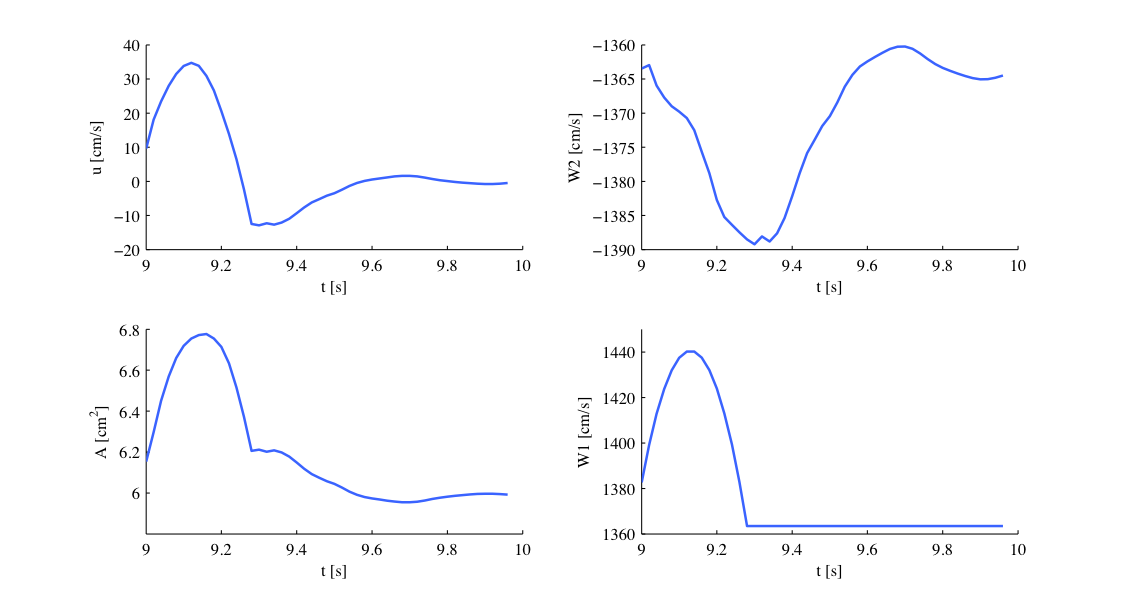
\includegraphics[width=\linewidth]{Figures/Network_Results.png}
\end{figure}

These short examples should give an insight to the functionality of our
PulseWaveSolver and show that results such as luminal area and pressure within
the artery can be simulated. These results can contribute to understanding the
physiology of the human vascular system and they can be used for
patient-specific planning of medical interventions.



\subsection{Stented Artery}
In the following we will explain the usage of the PulseWaveSolver on the basis
of a very common procedure in cardiovascular surgery: the placement of a stent
in an artery. Fig.~\ref{f:pulsewave:stent} (left) shows a schematic picture of a
stented artey, whereas Fig.~\ref{f:pulsewave:stent} (right) describes our
corresponding test-case layout.
\begin{figure}
	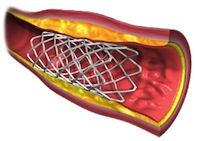
\includegraphics[width=0.35\linewidth]{Figures/stent_2.jpg}
	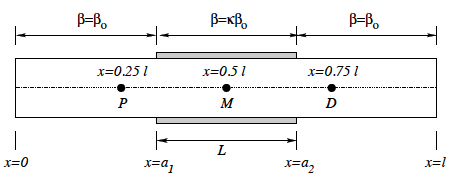
\includegraphics[width=0.6\linewidth]{Figures/P_M_D.png}
	\caption{}
	\label{f:pulsewave:stent}
\end{figure}
First we generate a one-dimensional inputfile called \inlsh{Test\_1.xml} by
defining vertices in the 3-dimensional space and connect them by segment elements. Here
we use $30$ elements and $31$ vertices respectively.

\subsubsection{Geometry}
In the following we desqcribe the geometry setup for modelling 1D flow in a
stent. This is done by defining vertices, elements and composites. The vertices
of the domain are shown in the following figure,

\begin{figure}
	\centering
	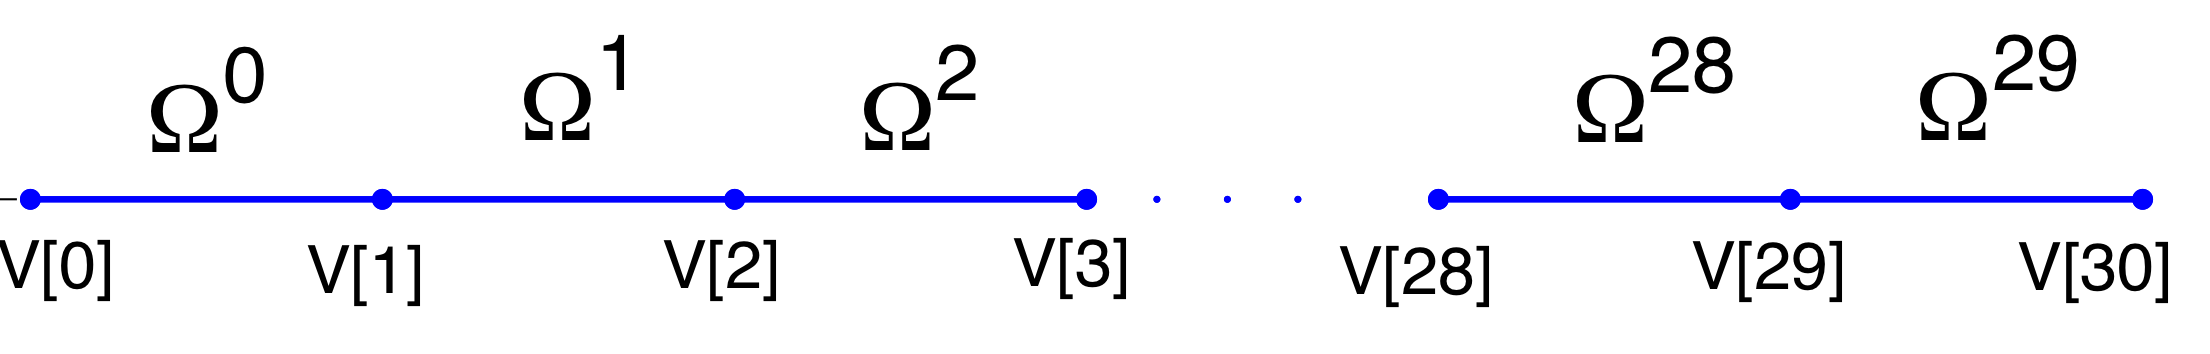
\includegraphics[width=\linewidth]{Figures/Domain.png}
\end{figure}

This is specified in the input file by,

\begin{lstlisting}[style=XmlStyle]
<VERTEX>
    <V ID="0"> 0.000e+00 0.000e+00 0.000e+00</V>
               .
               .
               . 
    <V ID="30">30.000e+00 0.000e+00 0.000e+00</V>
</VERTEX>
<ELEMENT>
    <S ID="0">    0     1 </S>
               .
               .
               . 
    <S ID="29">   29    30 </S>
</ELEMENT>
\end{lstlisting}

Then these elements are combined to three different composites, composite 0
represents all the elements, composite 1 the inflow boundary and composite 2 the
outflow boundary.

\begin{figure}
	\centering
	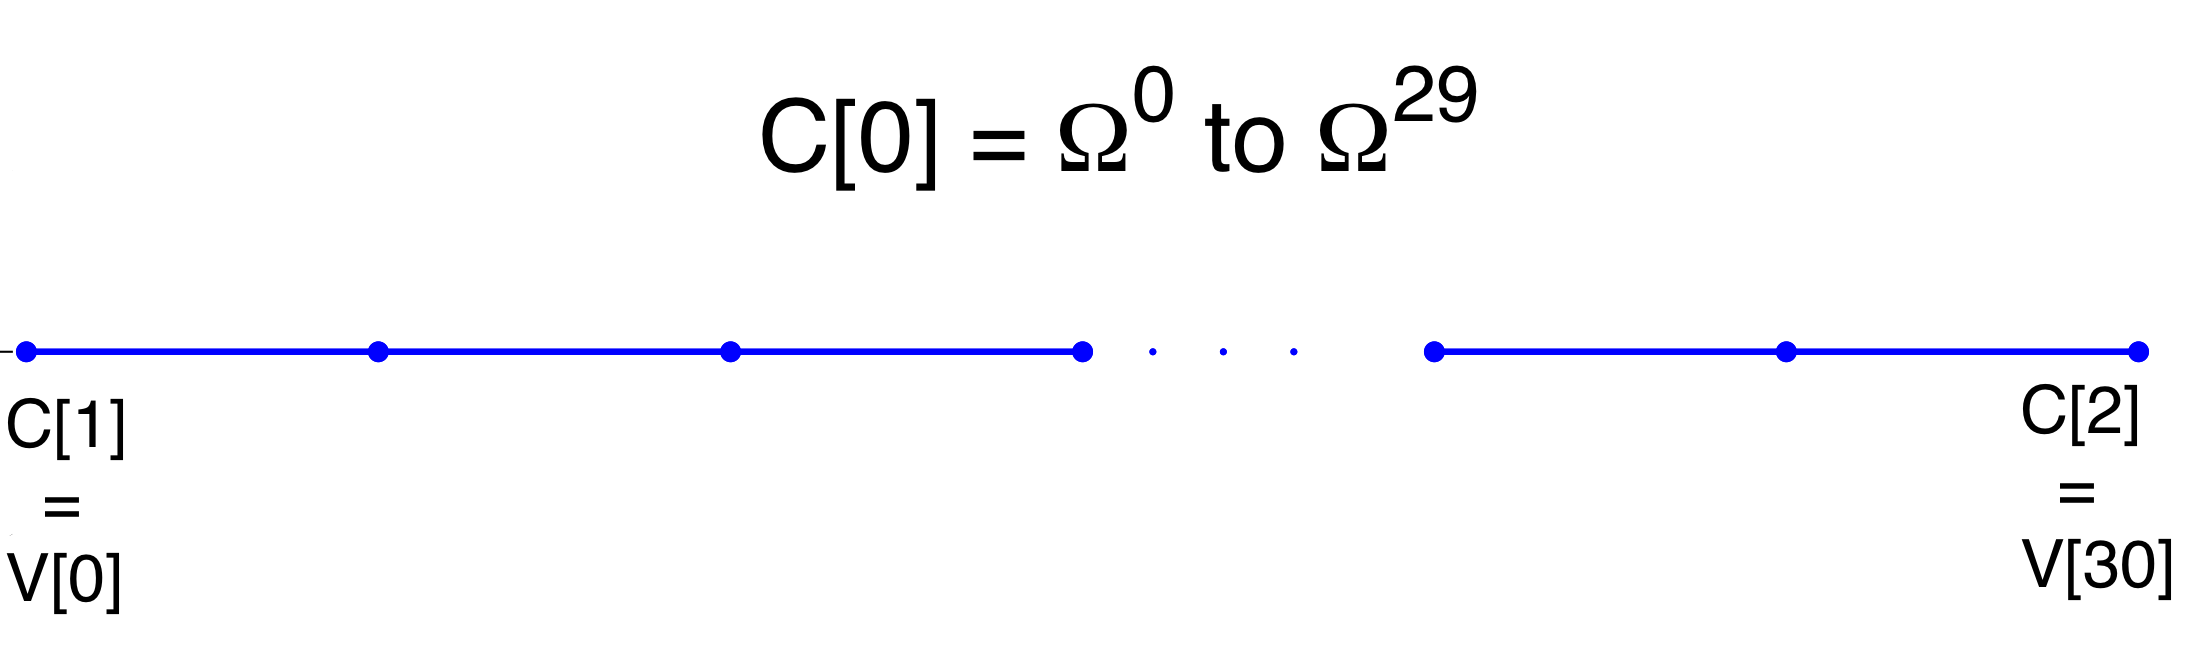
\includegraphics[width=\linewidth]{Figures/Composite.png}
\end{figure}

The above composites are specified as follows:
\begin{lstlisting}[style=XmlStyle]
<COMPOSITE>
    <C ID="0"> S[0-29] </C>
    <C ID="1"> V[0] </C>
    <C ID="2"> V[30] </C>
</COMPOSITE>
\end{lstlisting}

Finally the domain is specified by the first composite, via
\begin{lstlisting}[style=XmlStyle]
<DOMAIN> 
  <D ID="0"> C[0] </D>
</DOMAIN>
\end{lstlisting}

\subsubsection{Expansions}

For the expansions we use 4th-order polynomials which define our two variables A
and u on the domain.

\begin{lstlisting}[style=XmlStyle]
<EXPANSIONS>
  <E COMPOSITE="C[0]" NUMMODES="5" FIELDS="A,u" TYPE="MODIFIED" />
</EXPANSIONS>
\end{lstlisting}

\subsubsection{Parameters}

In the next section we provide all information that is required for the solution
of our biomedical flow problem such as: timestep, simulation time and several
parameters for the physics of our problem. The Discontinuous Galerkin
Method is used as projection scheme and the time-integration is performed by a
simple Forward Euler scheme.
\begin{lstlisting}[style=XmlStyle]
<PARAMETERS>
    <P> TimeStep       = 2e-6               </P>
    <P> FinTime        = 0.25               </P>
    <P> NumSteps       = FinTime/TimeStep   </P>
    <P> IO_CheckSteps  = NumSteps/50        </P>
    <P> IO_InfoSteps   = 100                </P>
    <P> T              = 0.33               </P>
    <P> h0             = 1.0                </P>
    <P> rho            = 1.0                </P>
    <P> nue            = 0.5                </P>
    <P> pext           = 0.0                </P>
    <P> a1             = 10.0               </P>
    <P> a2             = 20.0               </P>
    <P> kappa          = 100.0              </P>
    <P> Y0             = 1.9099e+5          </P>
    <P> k              = 2                  </P>
    <P> k1             = 200                </P>
</PARAMETERS>

<SOLVERINFO>
    <I PROPERTY="EQTYPE" VALUE="PulseWavePropagation" />
    <I PROPERTY="Projection" VALUE="DisContinuous" />
    <I PROPERTY="TimeIntegrationMethod" VALUE="ForwardEuler" />
    <I PROPERTY="UpwindTypePulse"  VALUE="UpwindPulse"/> 
</SOLVERINFO>

<VARIABLES>
    <V ID="0"> A </V>
    <V ID="1"> u </V>
</VARIABLES>
\end{lstlisting}

\begin{figure}
	\centering
	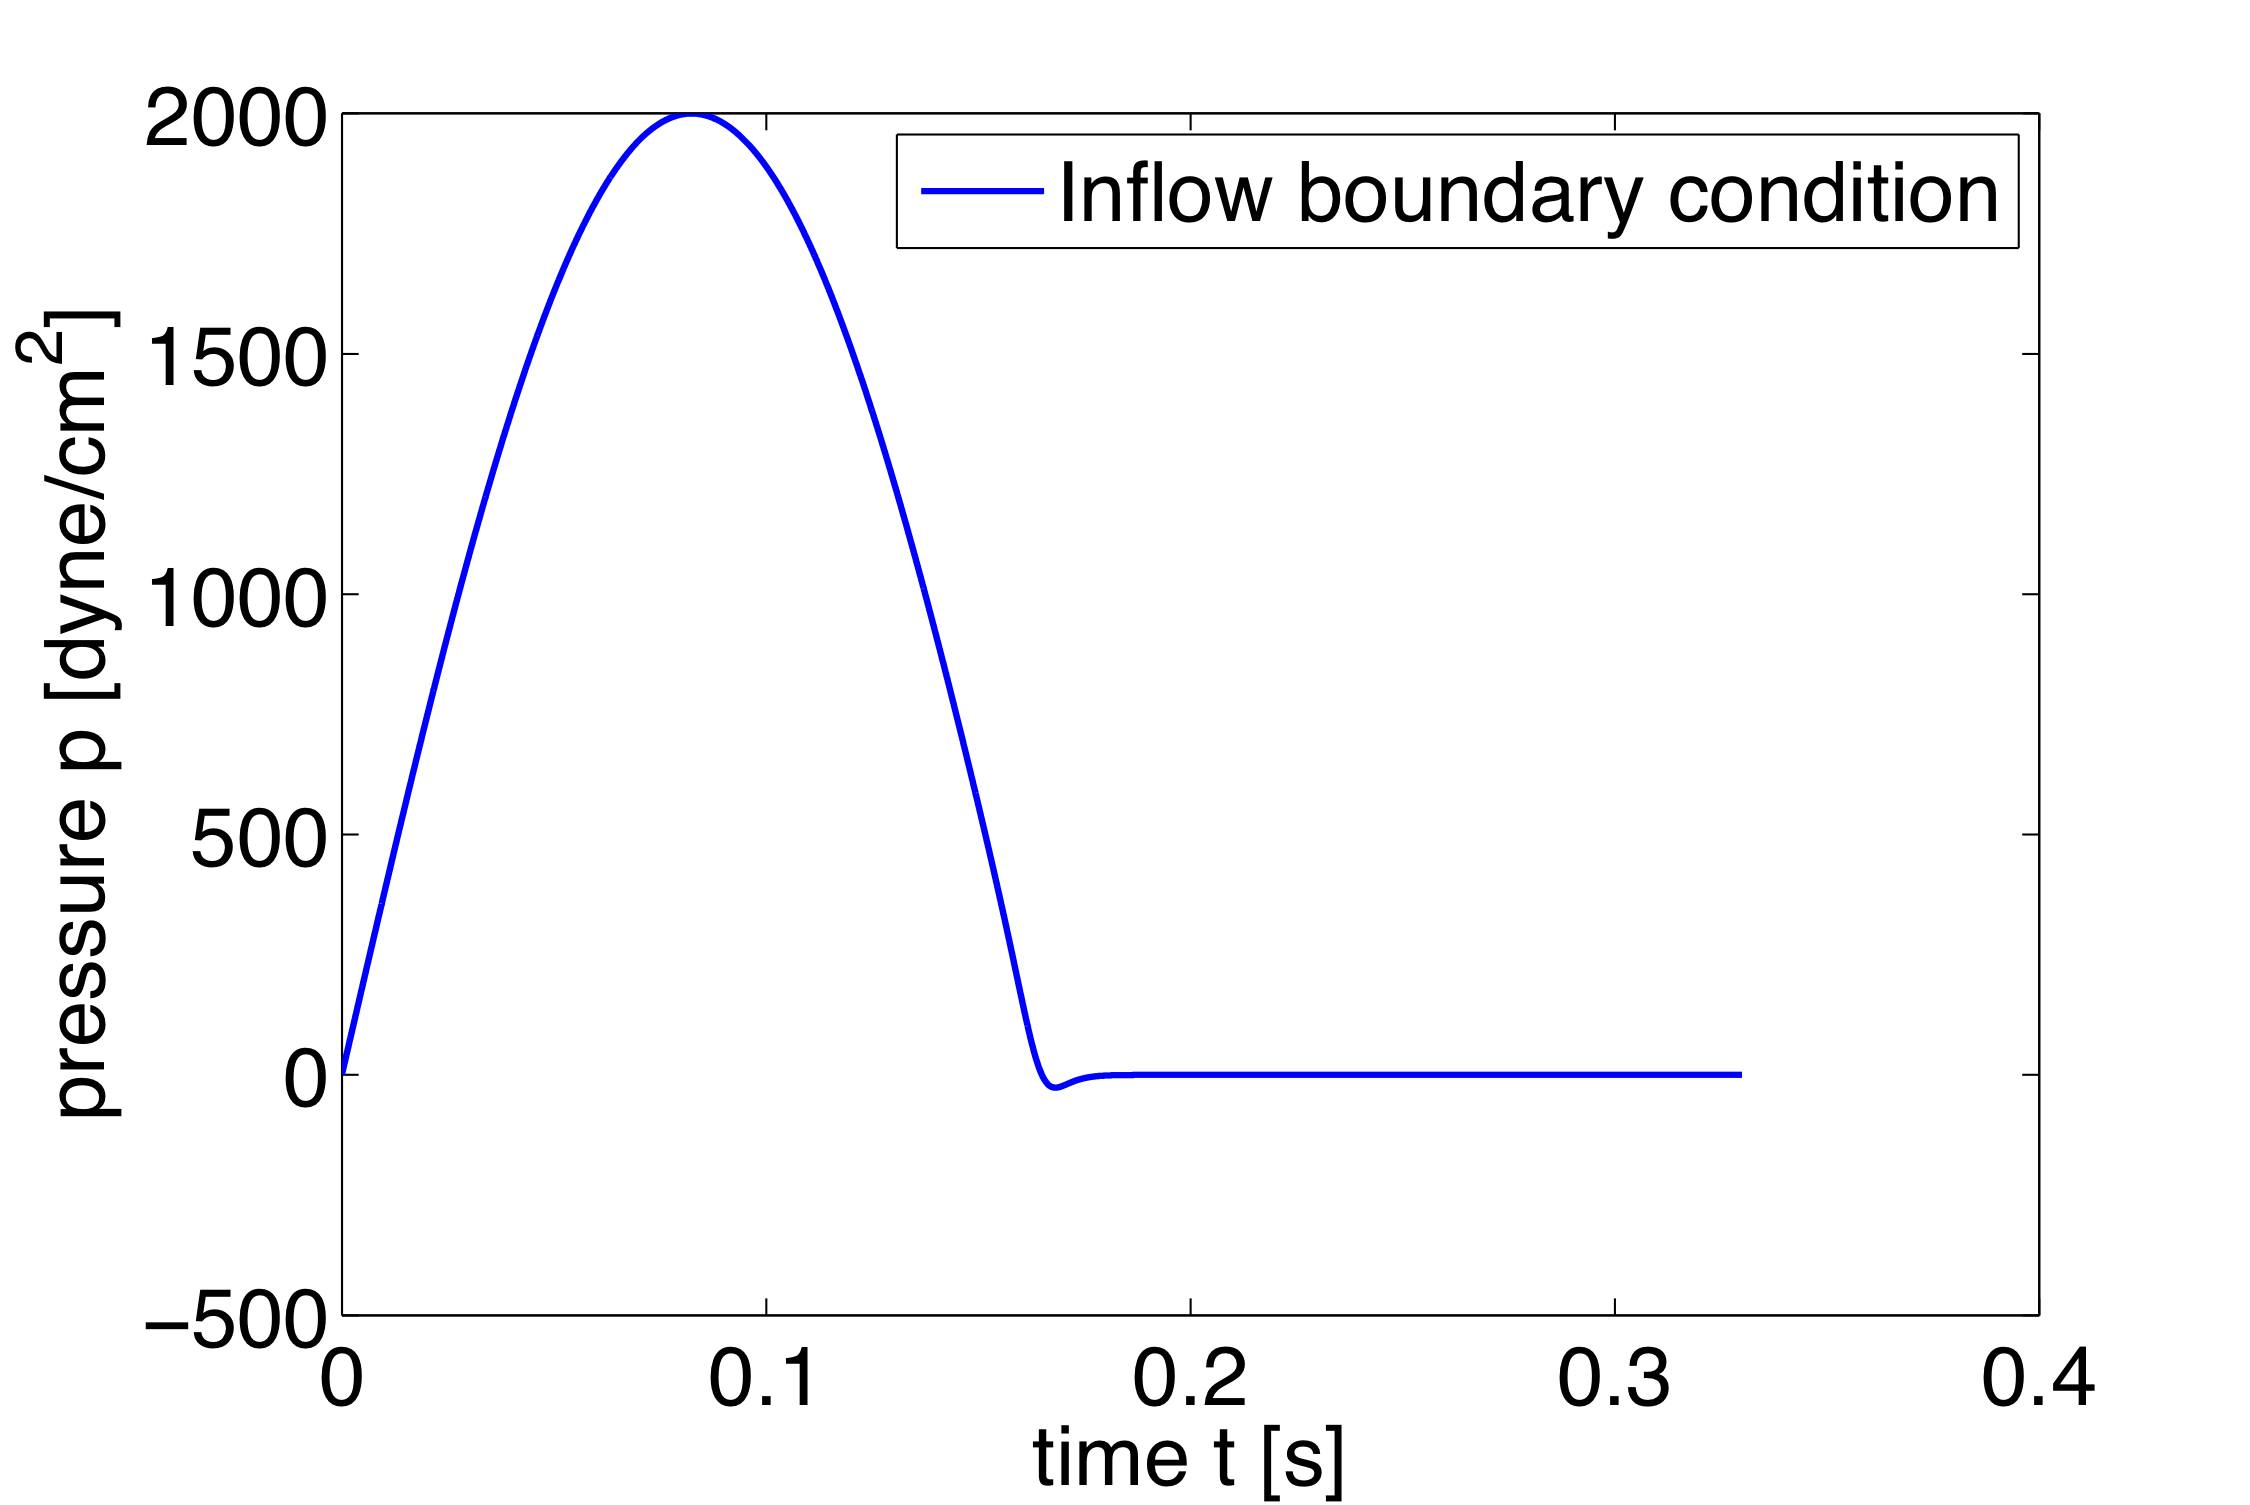
\includegraphics[width=0.49\linewidth]{Figures/Inflow.png}
	\caption{}
	\label{f:pulsewave:stented:inflow}
\end{figure}

\begin{figure}
	\centering
	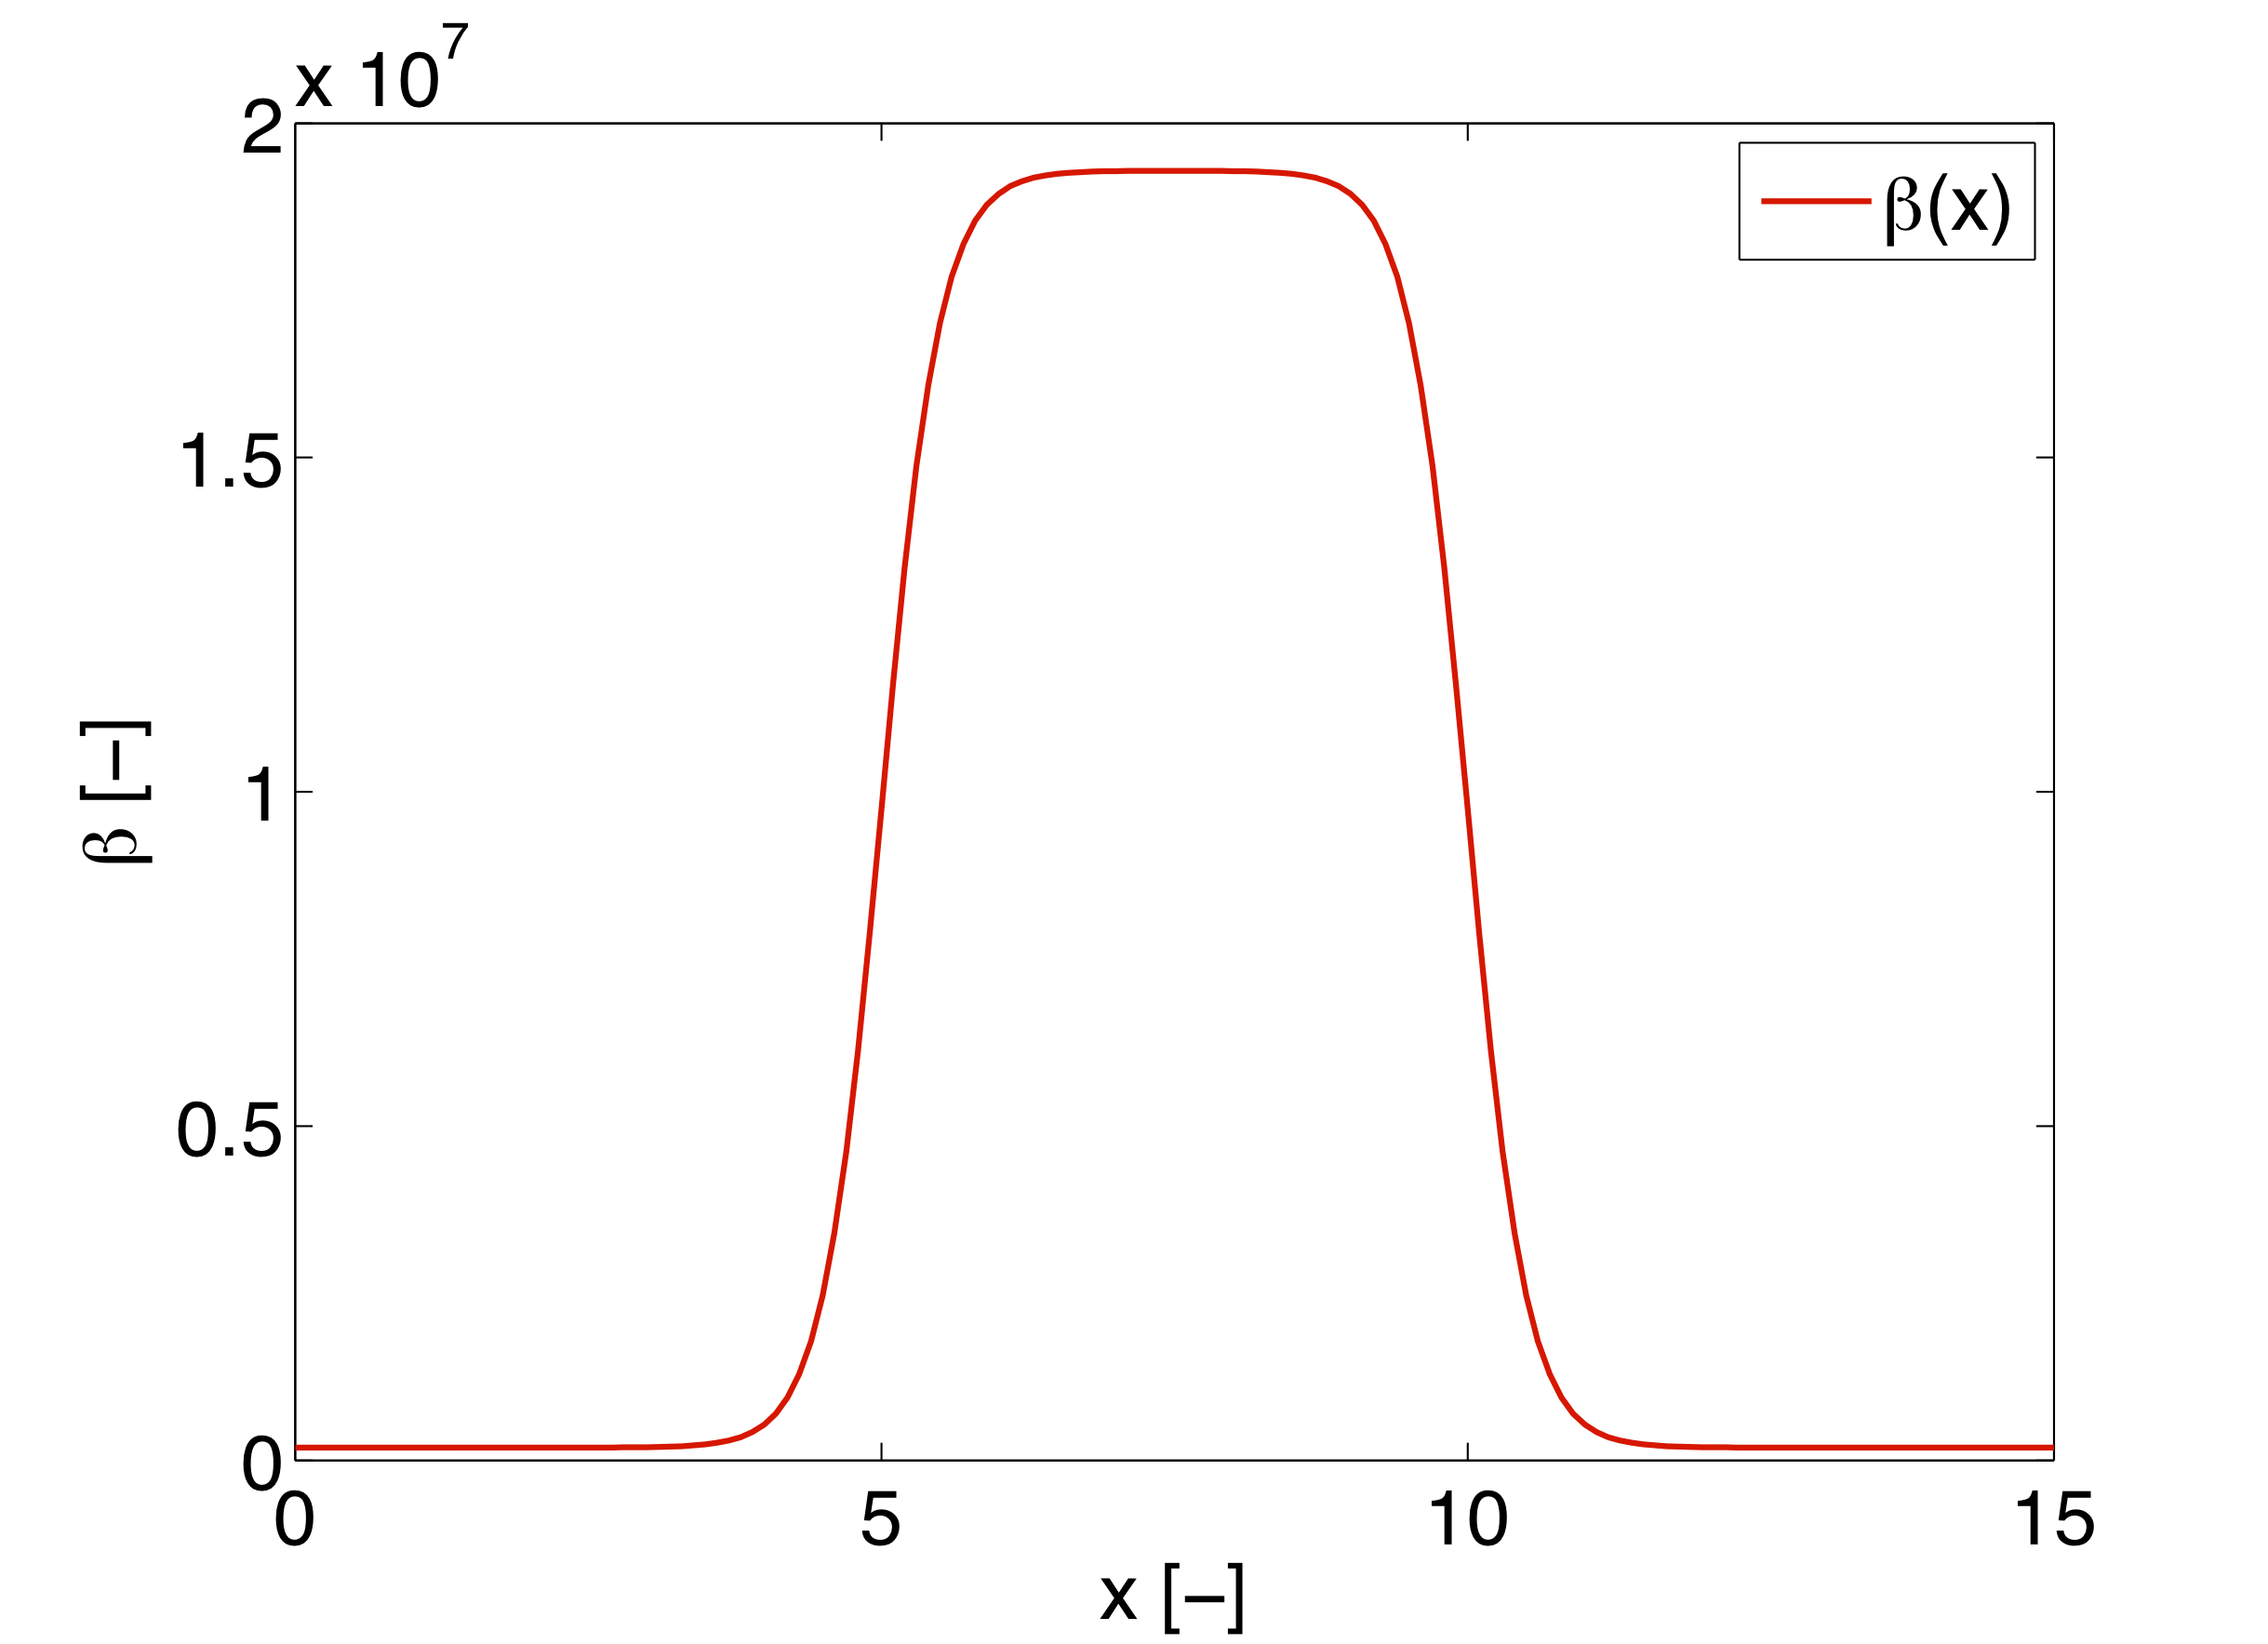
\includegraphics[width=0.49\linewidth]{Figures/betax.png}
	\caption{}
	\label{f:pulsewave:stented:betax}
\end{figure}

As for boundary conditions we apply a pressure boundary condition at the inflow
according to Fig.~\ref{f:pulsewave:stented:inflow}, modelling the pressure
variation during one heartbeat and a simple outflow boundary condition at the
right end of the tube.
\begin{lstlisting}[style=XmlStyle]
<BOUNDARYREGIONS>
    <B ID="0"> C[1] </B> <B ID="1"> C[2] </B>
</BOUNDARYREGIONS>

<BOUNDARYCONDITIONS>
    <REGION REF="0">
        <D VAR="A" USERDEFINEDTYPE="TimeDependent" 
           VALUE="(2000*sin(2*PI*t/T)*1./(1+exp(-2*k1*(T/2-t))-pext)/451352 +1)^2" /> 
        <D VAR="u" USERDEFINEDTYPE="TimeDependent" VALUE="1.0" />
    </REGION>
    <REGION REF="1">
        <D VAR="A" VALUE="1.0" />
        <D VAR="u" VALUE="1.0" />
    </REGION>
</BOUNDARYCONDITIONS>
\end{lstlisting}

Our simulation starts from the static equilibrium of the vessel with normalised
area and velocity. Also the area at the static equilibrium on the tube remains
constant at 1.0.
\begin{lstlisting}[style=XmlStyle]
<FUNCTION NAME="InitialConditions">
    <E VAR="A" DOMAIN="0" VALUE="1.0" /> 
    <E VAR="u" DOMAIN="0" VALUE="1.0" />
</FUNCTION>

<FUNCTION NAME="A_0">
    <E VAR="A" DOMAIN="0" VALUE="1.0" />
</FUNCTION>
\end{lstlisting}

We will apply the stent by introducing a discontinuity in the material
properties following the graph in Fig.~\ref{f:pulsewave:stented:betax}. To run
the simulation without stent we just set \inltt{E0=Y0}.
\begin{lstlisting}[style=XMLStyle]
<FUNCTION NAME="MaterialProperties"> 
    <E VAR="E0" DOMAIN="0" 
       VALUE="Y0*(1.0-kappa/(1+exp(-2*k*(a1-x)))+kappa/(1+exp(-2*k*(a2-x))))" />
</FUNCTION>
\end{lstlisting}

\subsubsection{Simulation}
The simulation is started by running
\begin{lstlisting}[style=BashInputStyle]
PulseWaveSolver Test_1.xml
\end{lstlisting}
It will take about 60 seconds on a 2.4GHz Intel Core 2 Duo processor and 
therefore is computationally realisable at every clinical site.

\subsubsection{Results}
As a result we get a 3-dimensional interpretation of the aortic cross-sectional
area varying in axial direction both for the stented and non-stented vessel. In
case of the stent, the rigid metal mesh will restrict the deformation of the
area in that specific part of the artery compared to the normal vessel
(Fig.~\ref{f:pulsewave:stented:vessels}).

\begin{figure}
	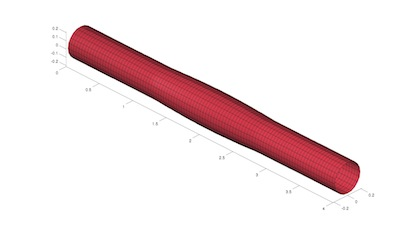
\includegraphics[width=0.49\linewidth]{Figures/normal_vessel.jpg}
	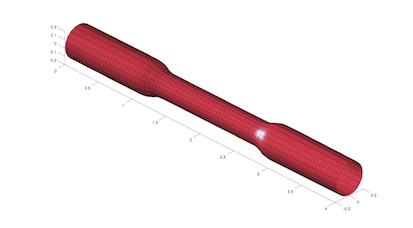
\includegraphics[width=0.49\linewidth]{Figures/stented_vessel.jpg}
	\caption{}
	\label{f:pulsewave:stented:vessels}
\end{figure}

Also, if we look at the pressure at three points within the artery (P, M, D) we
will recognize that there are major differences between the stented and normal
vessel. While in the normal vessel (left) the pressure wave applied at the
inflow is propagated without any losses, this does not hold for the stented
artery (right). Here, the stiffening at the stent causes reflections and thus
there are losses for total pressure at the medial (M) and distal (D) point.

\begin{figure}
	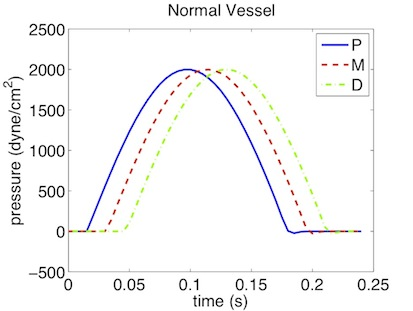
\includegraphics[width=0.49\linewidth]{Figures/pressure_normal_vessel.jpg}
	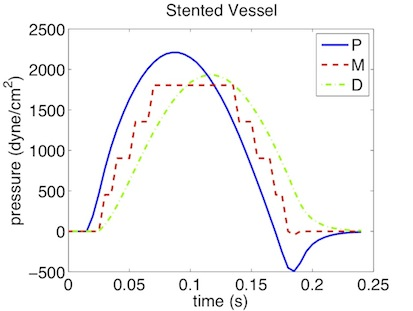
\includegraphics[width=0.49\linewidth]{Figures/pressure_stented_vessel.jpg}
\end{figure}

\section{Further Information}
The PulseWaveSolver has beqen developed with contributions by various students
and researchers at the Department of Aeronautics, Imperial College London. 
Further information on the solver and its underlying mathematical framework 
can be found in \cite{Ro12,Pi12}.

\section{Future Development}
The PulseWaveSolver is a useful tool for computational modelling of
one-dimensional blood flow in the human body. However, there are several ideas
for future development which include:
\begin{enumerate}
\item Inclusion of a pre-processor and post-processor.
\item Profiling the code to improve performance.
\item Cleaning up the input file to make the input format more user-friendly.
\item Modelling of valves and alternative pressure-area laws for models of
venous flow.
\item Incorporating a model of the heart.
\end{enumerate}

% These are unreferenced citations
% J. Alastruey, Numerical modelling of pulse wave propagation in the
 % cardiovascular system: development, validation and clinical applications, PhD thesis, 2006
% N. Westerhof et al., Anatomic studies of the human systemic arterial tree, J.
% Biomech. 2:121-143, 1969 Three-dimensional blood flow profile in a rabbit aorta done with Nektar++,
% courtesy of Véronique Peiffer 
